\documentclass[a4paper]{article}
\usepackage[T1]{fontenc}			% pacchetto per \chapter
\usepackage[italian]{babel}
\usepackage[italian]{isodate}  		% formato delle date in italiano
\usepackage{graphicx}				% gestione delle immagini
\usepackage{amsfonts}
\usepackage{booktabs}				% tabelle di qualità superiore
\usepackage{amsmath}				% pacchetto matematica
\usepackage{mathtools}				% per sottolineare sotto le equazioni
\usepackage{stmaryrd} 				% per '\llbracket' e '\rrbracket'
\usepackage{amsthm}					% teoremi migliorati
\usepackage{enumitem}				% gestione delle liste
\usepackage{pifont}					% pacchetto con elenchi carini
\usepackage{enumitem}				% pacchetto per elenchi con lettere dell'alfabeto
\usepackage{cancel}					% per cancellare delle espressioni matematiche
\usepackage{caption}				% caption personalizzati
\usepackage[]{mdframed}				% box per il testo
\usepackage{multirow}				% più linee in una tabella
\usepackage{gensymb}				% simbolo di degree
\usepackage{listings}				% pacchetto per i codici

% draw a frame around given text
\newcommand{\framedtext}[1]{%
	\par%
	\noindent\fbox{%
		\parbox{\dimexpr\linewidth-2\fboxsep-2\fboxrule}{#1}%
	}%
}



\usepackage[x11names]{xcolor}		% pacchetto colori RGB
% Link ipertestuali per l'indice
\usepackage{xcolor}
\usepackage[linkcolor=black, citecolor=blue, urlcolor=cyan]{hyperref}
\hypersetup{
	colorlinks=true
}

\usepackage{tikz}
\newcommand{\MyTikzmark}[2]{%
	\tikz[overlay,remember picture,baseline] \node [anchor=base] (#1) {#2};%
}
\newcommand{\DrawVLine}[3][]{%
	\begin{tikzpicture}[overlay,remember picture]
		\draw[shorten <=0.3ex, #1] (#2.north) -- (#3.south);
	\end{tikzpicture}
}
\newcommand{\DrawHLine}[3][]{%
	\begin{tikzpicture}[overlay,remember picture]
		\draw[shorten <=0.2em, #1] (#2.west) -- (#3.east);
	\end{tikzpicture}
}


%\usepackage{showframe}				% visualizzazione bordi
%\usepackage{showkeys}				% visualizzazione etichetta

\newtheorem{theorem}{\textcolor{Red3}{\underline{Teorema}}}
\newtheorem{lemma}{Lemma}
\renewcommand{\qedsymbol}{QED}
\newcommand{\exec}[1]{\llbracket #1\:\rrbracket}
\newcommand{\dquotes}[1]{``#1''}
\newcommand{\longline}{\noindent\rule{\textwidth}{0.4pt}}
\newcommand{\circledtext}[1]{\raisebox{.5pt}{\textcircled{\raisebox{-.9pt}{#1}}}}

\newenvironment{rowequmat}[1]{\left(\array{@{}#1@{}}}{\endarray\right)}
\newenvironment{rowequmatbra}[1]{\left[\array{@{}#1@{}}}{\endarray\right]}

\definecolor{codegreen}{rgb}{0,0.6,0}
\definecolor{codegray}{rgb}{0.5,0.5,0.5}
\definecolor{codepurple}{rgb}{0.58,0,0.82}
\definecolor{backcolour}{rgb}{0.95,0.95,0.92}
\lstdefinestyle{mystyle}{
	backgroundcolor=\color{backcolour},   
	commentstyle=\color{codegreen},
	keywordstyle=\color{magenta},
	numberstyle=\tiny\color{codegray},
	stringstyle=\color{codepurple},
	basicstyle=\ttfamily\footnotesize,
	breakatwhitespace=false,         
	breaklines=true,                 
	captionpos=b,                    
	keepspaces=true,                 
	numbers=left,                    
	numbersep=5pt,                  
	showspaces=false,                
	showstringspaces=false,
	showtabs=false,                  
	tabsize=2
}

\lstset{style=mystyle}

\begin{document}
	\author{VR443470}
	\title{Guida agli Esami di Linguaggi}
	\date{\printdayoff\today}
	\maketitle
	
	\newpage
	
	% indice
	\tableofcontents
	
	\newpage
	
	\section{Esercizio 1 - Domanda di teoria su Interprete e Compilatore}
	
	\subsection{Interprete}
	
	In molti esami si presenta la richiesta della definizione di interprete. Nonostante possa essere banale, viene richiesto un \dquotes{alto} livello di approfondimento dato che vale ben 4 punti all'interno dell'esame. In ogni caso, è possibile affermare che questa domanda sia una delle più gettonate.\newline
	
	\noindent
	\textcolor{Red3}{\textbf{\emph{Definire intuitivamente e formalmente (mediante definizione semantica) cosa è un interprete. Descrivere la struttura di un interprete e spiegarne il funzionamento.}}}\newline
	
	\noindent
	\textcolor{Green4}{\textbf{\emph{\underline{Risposta}}}}\newline
	
	\noindent
	La definizione intuitiva di un interprete è la seguente.
	
	Un \textbf{interprete} è un programma $\mathrm{int}^{L_{0}, L}$ che esegue, sulla macchina astratta per $L_{0}$, programmi $P^{L}$, i quali sono scritti nel linguaggio di programmazione $L$, su un input fissato appartenente all'insieme dei dati $D$ (input e output).\newline
	Utilizzando parole povere, un interprete non è altro che una \dquotes{macchina universale} che preso un programma e un suo input, esegue (il programma) sul quel determinato input usando \underline{soltanto} le funzionalità messe a disposizione dal livello (macchina astratta) sottostante.
	\begin{mdframed}
		\emph{Un attimo, ma che cosa si intende per livello? E macchina astratta?} Cerchiamo di fare chiarezza.\newline
		
		\noindent
		Dato un linguaggio di programmazione $L$, la \underline{macchina astratta} $M_{L}$ per $L$ è un insieme di strutture dati ed algoritmi che consentono di memorizzare ed eseguire programmi scritti in $L$. La sua realizzazione può essere fatta in Hardware, Firmware o Software.\newline
		
		\noindent
		\emph{Si ma quindi cosa si intende per livello?}\newline
		
		\noindent
		Con la scelta della categoria \dquotes{realizzazione software}, vengono utilizzati, per la realizzazione di strutture dati e algoritmi, linguaggi di programmazione ad alto livello poiché essi implementano una struttura suddivisa a \underline{livelli} di astrazione.\newline
		Per concludere, la macchina astratta può essere dunque vista come una stratificazione di livelli dove ciascuno di essi coopera in modo sequenziale, ma allo stesso tempo è indipendente.\newline
		
		\noindent
		Per non lasciare niente al caso, con \dquotes{\underline{linguaggio di programmazione ad alto} \underline{livello}} ci si riferisce a tutti quei linguaggi di programmazione che offrono un livello di astrazione molto alto dei dettagli del funzionamento del calcolatore.
	\end{mdframed}\newpage
	
	\noindent
	Prima della definizione formale di interprete, si illustrano due notazioni necessarie:
	\begin{itemize}
		\item Con il termine $Prog^{L}$ ci si riferisce all'insieme dei programmi scritti nel linguaggio di programmazione $L$;
		
		\item Con la dicitura:
		\begin{equation*}
			\exec{P^{L}} \: : \: D \rightarrow D
		\end{equation*}
		Si indica che l'esecuzione del programma scritto nel linguaggio di programmazione $L$ ($\exec{P^{L}}$) con input $in$ è uguale all'output $out$. Ovverosia:
		\begin{equation*}
			\exec{P^{L}}\left(in\right) = out	
		\end{equation*}
	\end{itemize}
	Un \textbf{interprete formalmente} è descrivibile nel seguente modo. Si consideri un interprete da $L$ a $L_{0}$: dato $P^{L} \in Prog^{L}$ e $in \in D$, un interprete $int^{L, L_{0}}$ per $L$ su $L_{0}$ è un programma tale che:
	\begin{equation*}
		\exec{int^{L, L_{0}}} \: : \: \left(Prog^{L}\right) \rightarrow D
	\end{equation*}
	Ne consegue che:
	\begin{equation*}
		\exec{int^{L, L_{0}}} \: : \: \left(P^{L}, in\right) = \exec{P^{L}}\left(in\right)
	\end{equation*}
	\begin{figure}[!htp]
		\centering
		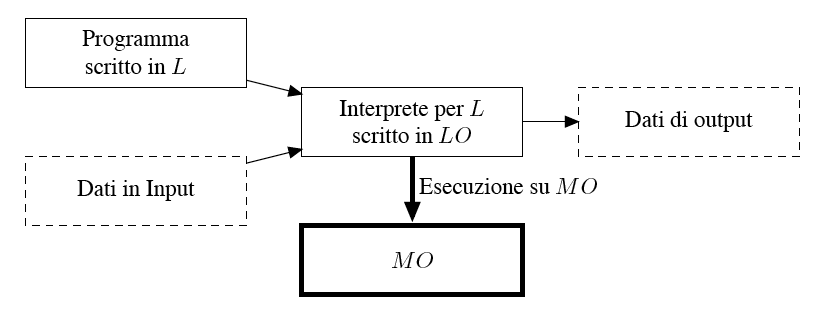
\includegraphics[width=\textwidth]{img/ex1-1.png}
		\caption*{Riassunto visivo di quanto appena descritto.}
	\end{figure}\newpage
	
	\noindent
	Qua di seguito si presenta il ciclo di esecuzione di un interprete:
	\begin{figure}[!htp]
		\centering
		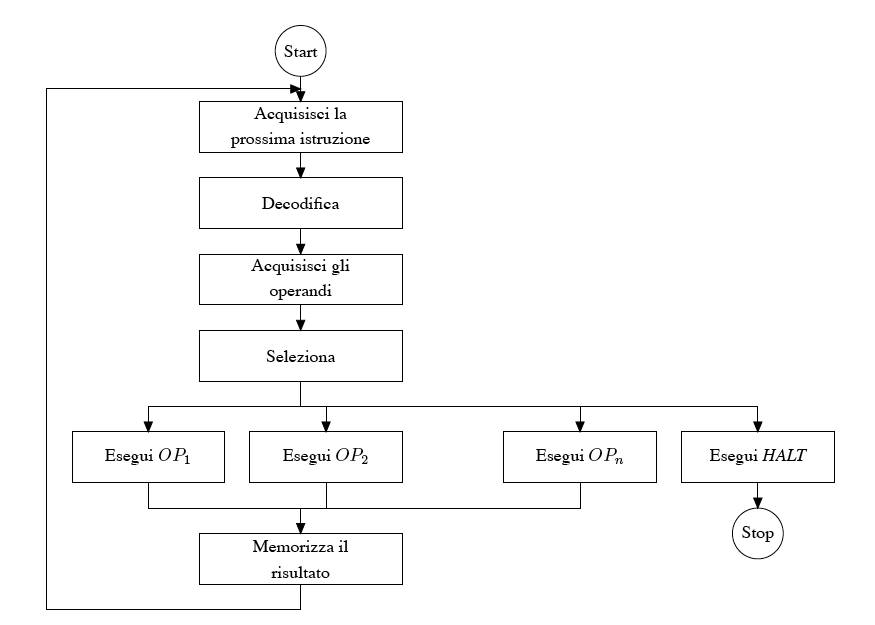
\includegraphics[width=\textwidth]{img/ex1-2.png}
	\end{figure}
	\begin{enumerate}
		\item Il ciclo di esecuzione di un interprete si apre con l'acquisizione di un'istruzione da eseguire;
		
		\item L'operazione del passo precedente viene decodificata;
		
		\item Nel caso in cui l'operazione abbia bisogno di operandi, anch'essi vengono acquisiti dalla memoria;
		
		\item Data l'operazione acquisita al passo 1, viene selezionata una determinata operazione: nel caso di $OP_{...}$ si esegue un'operazione, nel caso di $HALT$ l'esecuzione di un interprete si ferma;
		
		\item Dopo l'operazione eseguita, se vi è un risultato, esso viene salvato. In ogni caso, il ciclo inizia nuovamente la sua esecuzione.
	\end{enumerate}
	
	\newpage
	\subsection{Compilatore}
	
	Non è frequente la richiesta della definizione di compilatore, ma rimane una domanda di teoria che può essere richiesta.\newline
	
	\noindent
	\textcolor{Red3}{\textbf{\emph{Definire intuitivamente e formalmente (mediante definizione semantica) cosa è un compilatore. Descrivere e spiegare poi la struttura di un compilatore (preferibilmente come flow-chart).}}}\newline
	
	\noindent
	\textcolor{Green4}{\textbf{\emph{\underline{Risposta}}}}\newline
	
	\noindent
	La definizione intuitiva di un compilatore è la seguente.
	
	Un \textbf{compilatore} è un programma $comp^{L_{0},L}$ che traduce, preservando semantica e funzionalità, programmi scritti nel linguaggio di programmazione $L$ in programmi scritti in $L_{0}$, e quindi eseguibili direttamente sulla macchina astratta per $L_{0}$.\newline
	
	\noindent
	Dato un linguaggio di programmazione $L$, una macchina astratta $M_{L}$ per $L$ è un insieme di strutture dati e algoritmi che consentono la memorizzazione e l'esecuzione dei programmi scritti nel linguaggio di programmazione $L$ ($P^{L}$).\newline
	
	\noindent
	Prima di dare la definizione formale di interprete, si forniscono alcune notazioni:
	\begin{itemize}
		\item $Prog^{L}$ è un insieme di programmi scritti nel linguaggio di programmazione $L$;
		\item $D$ è l'insieme dei dati (input e output);
		\item $P^{L}$ è il programma scritto nel linguaggio di programmazione $L$;
		\item $\exec{P^{L}} \: : \: D \rightarrow D$ rappresenta la semantica di $P^{L}$, ovvero l'esecuzione del programma nel linguaggio di programmazione $L$ con input $in$ è uguale all'output $out$:
		\begin{equation*}
			\exec{P^{L}}(in) = (out)
		\end{equation*}
	\end{itemize}
	La definizione formale di un compilatore è la seguente.
	
	Dato $P^{L} \in Prog^{L}$, un \textbf{compilatore formalmente} $comp^{L,L_{0}}$ da $L$ a $L_{0}$ è un programma che:
	\begin{equation*}
		\exec{comp^{L,L_{0}}}: Prog^{L} \rightarrow Prog^{L_{0}}
	\end{equation*}
	Ovvero:
	\begin{equation*}
		\exec{comp^{L,L_{0}}}\left(P^{L}\right) = \left(P^{L_{0}}\right) \hspace{1em} \text{tale che} \hspace{1em} \forall in \in D.\exec{P^{L_{0}}}\left(in\right) = \exec{P^{L}}\left(in\right)
	\end{equation*}
	In linguaggio non matematico, significa che l'esecuzione del compilatore da $L$ a $L_{0}$ insieme (input) ad un determinato programma scritto in un linguaggio di programmazione $L$ è uguale (output) al programma scritto nel linguaggio di programmazione $P^{L_{0}}$; tale che per ogni input $in$ appartenente all'insieme dei dati $D$, l'esecuzione di un programma scritto nel linguaggio di programmazione $L_{0}$ con input $in$ è uguale all'esecuzione del programma scritto nel linguaggio di programmazione $L$ con input $in$.\newpage
	
	\begin{figure}[!htp]
		\centering
		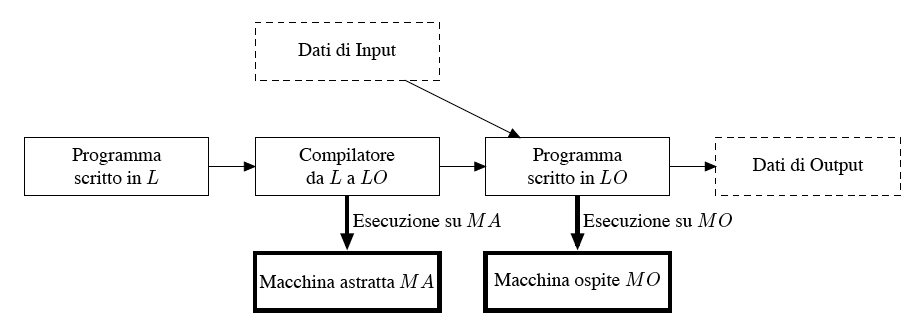
\includegraphics[width=\textwidth]{img/ex1-3.png}
		\caption*{Flow-chart di quanto detto precedentemente.}
	\end{figure}
	
	\noindent
	Si presenta qua di seguito la \textbf{struttura di un compilatore}:
	\begin{figure}[!htp]
		\centering
		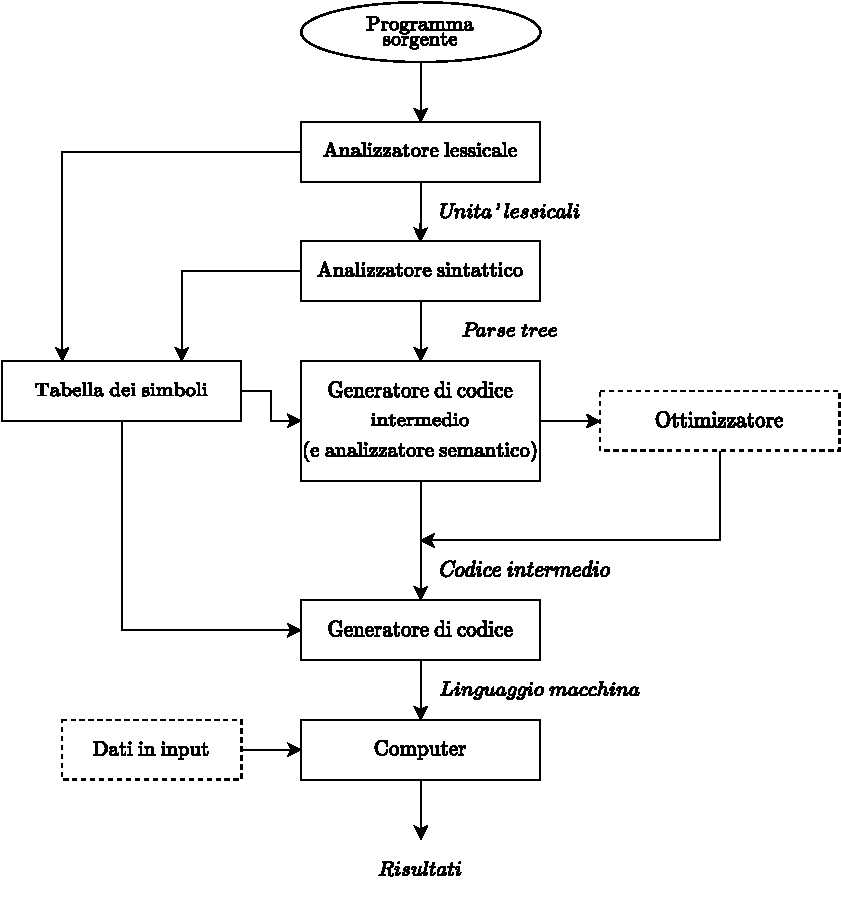
\includegraphics[width=\textwidth]{img/ex1-4.pdf}
	\end{figure}\newpage
	
	\begin{enumerate}
		\item Il programma sorgente, da compilare, passa in prima battuta da un analizzatore lessicale. Vengono \textbf{convertiti i caratteri del programma sorgente in unità lessicali}. Quest'ultime possono essere \emph{identificatori}, \emph{numeri}, \emph{parole riservate} e formano i linguaggi regolari.
		
		\item Le unità lessicali finiscono in un analizzatore sintattico, il quale crea una albero che rappresenta la sintassi del programma:
		\begin{itemize}
			\item Le foglie (\emph{token}) vengono lette da sinistra verso destra e costituiscono le frasi ben formate del linguaggio;
			
			\item Dal precedente punto, ne consegue che l'impossibilità della costruzione di un albero è dovuta all'illegalità di quale frase (mal formata, errore di compilazione!);
		\end{itemize}
		Quindi, l'\textbf{analizzatore sintattico trasforma unità lessicali in \emph{parse tree} (albero di parse) che rappresentano la struttura sintattica del programma}.
		
		\item Riceve informazioni dall'analizzatore lessicale/sintattico e \textbf{memorizza informazioni sui nomi presenti nel programma} (identificatori, chiamate di procedura, ecc.);
		
		\item A questo punto, viene \textbf{generato un codice intermedio} che è \emph{indipendente dall'architettura}, e vengono \textbf{rilevati eventuali errori semantici} grazie all'\emph{analizzatore semantico};
		
		\item (Opzionale) Il codice può essere ottimizzato in questa fase;
		
		\item Si conclude la struttura del compilatore con la generazione del codice macchina che, a differenza del codice intermedio, è dipendente dall'architettura.
	\end{enumerate}
	La parte finale dello schema mostra l'esecuzione del programma compilato su un computer con eventuali dati in input.\newpage
	
	\section{Esercizio 2 - Induzione}
	
	\subsection{Dimostrare $\forall n \in \mathbb{N}.n + n^{2}$ è un numero pari}
	
	\textcolor{Red3}{\textbf{\emph{Dimostrare per induzione che $\forall n \in \mathbb{N}.n + n^{2}$ è un numero pari.}}}\newline
	
	\noindent
	\textcolor{Green4}{\textbf{\emph{\underline{Risposta}}}}\newline
	
	\noindent	
	L'\textbf{induzione} è una tecnica di dimostrazione che consente di dimostrare la validità di una tesi dalla verifica di due condizioni: la validità della \dquotes{base induttiva} e la validità del \dquotes{passo induttivo}.
	\begin{proof}[\textbf{Caso base}]
		Si sceglie come caso base il valore $n = 1$. Si sostituisce:
		\begin{equation*}
			\begin{array}{rcl}
				n + n^{2} &\rightarrow& \text{ è pari? } \textcolor{Green4}{\checkmark} \\ [.3em]
				&\downarrow& \text{sostituzione di }n=1 \\ [.3em]
				1 + 1^{2} = 2 &\rightarrow& \text{ è pari? } \textcolor{Green4}{\checkmark}
			\end{array}
		\end{equation*}
		Utilizzando un linguaggio più formale, utile per la dimostrazione, è anche possibile affermare che il modulo di $n+n^{2}$ diviso $2$ è uguale a zero. Ovvero, che dividendo un numero pari per $2$ (per definizione), si ottiene il valore zero:
		\begin{equation*}
			\begin{array}{rcl}
				n+n^{2} &=& 0 \: \left(\mathrm{mod} \: 2\right) \\ [.3em]
				%
				&\downarrow& \text{sostituzione di }n=1 \\ [.3em]
				%
				1+1^{2} &=& 0 \: \left(\mathrm{mod} \: 2\right)
			\end{array}
		\end{equation*}
	\end{proof}
	
	\noindent
	\textbf{\emph{Ipotesi induttiva:}} si assume che sia vera:
	\begin{equation*}
		n+n^{2} = 0 \: \left(\mathrm{mod} \: 2\right) \hspace{1em} \forall n \in \mathbb{N}
	\end{equation*}
	
	\begin{proof}[\textbf{Passo induttivo}]
		Si dimostra che l'ipotesi induttiva implica la validità della proprietà per $n+1$:
		\begin{equation*}
			\begin{array}{rcl}
				n+n^{2} &=& 0 \: \left(\mathrm{mod} \: 2\right) \\ [.3em]
				%                                                       
				&\downarrow& \text{applico passo induttivo} \\ [.3em]    
				%
				n+1 + \left(n+1\right)^{2} &=& 0 \: \left(\mathrm{mod} \: 2\right) \\ [.3em]
				%
				n + 1 + n^{2} + 2n + 1 &=& 0  \: \left(\mathrm{mod} \: 2\right) \\ [.3em]
				%
				n^{2} + n + 2n + 2 &=& 0 \: \left(\mathrm{mod} \: 2\right) \\ [.3em]
				%
				&\downarrow& \text{applico l'ipotesi induttiva} \\ [.3em]
				%
				n^{2} + n + 2n + 2 &=& n^{2} + n \\ [.3em]
				%
				2n + 2 &=& 0 \: \left(\mathrm{mod} \: 2\right)
			\end{array}
		\end{equation*}
		Per definizione:
		\begin{itemize}
			\item Qualsiasi numero moltiplicato per $2$ si ottiene un numero pari;
			\item Il risultato tra la somma di due numeri pari è ancora un numero pari;
			\item $2$ è un numero pari.
		\end{itemize}
	\end{proof}\newpage
	
	\subsection{Dimostrare $\displaystyle\sum_{i=1}^{n}\dfrac{1}{i\left(i+1\right)} = \dfrac{n}{n+1}$}
	\textcolor{Red3}{\textbf{\emph{Dimostrare per induzione che }}$\displaystyle\sum_{i=1}^{n}\dfrac{1}{i\left(i+1\right)} = \dfrac{n}{n+1}$\textbf{\emph{.}}}\newline
	
	\noindent
	\textcolor{Green4}{\textbf{\emph{\underline{Risposta}}}}\newline
	
	\noindent
	L'\textbf{induzione} è una tecnica di dimostrazione che consente di dimostrare la validità di una tesi dalla verifica di due condizioni: la validità della \dquotes{base induttiva} e la validità del \dquotes{passo induttivo}.
	\begin{proof}[\textbf{Caso base}]
		Si sceglie come caso base il valore $n = 1$. Quindi, si va a sostituire:
		\begin{equation*}
			\begin{array}{rcl}
				\displaystyle\sum_{i=1}^{n}\dfrac{1}{i\left(i+1\right)} &=& \dfrac{n}{n+1} \\ [1.5em]
				%
				&\downarrow& \text{sostituzione }n=1 \\ [.5em]
				%
				\displaystyle\sum_{i=1}^{1}\dfrac{1}{i\left(i+1\right)} &=& \dfrac{1}{1+1} \\ [1.5em]
				%
				&\downarrow& \text{calcolo della sommatoria} \\ [.5em]
				%
				\displaystyle\sum_{i=1}^{1}\dfrac{1}{1\left(1+1\right)} &=& \dfrac{1}{1+1} \\ [1.5em]
				%
				\dfrac{1}{2} &=& \dfrac{1}{2}
			\end{array}
		\end{equation*}
	\end{proof}
	
	\noindent
	\textbf{\emph{Ipotesi induttiva:}} si assume che sia vera:
	\begin{equation*}
		\displaystyle\sum_{i=1}^{n}\dfrac{1}{i\left(i+1\right)} = \dfrac{n}{n+1} \hspace{2em} \forall n
	\end{equation*}
	
	\begin{proof}[\textbf{Passo induttivo}]
		Si dimostra che l'ipotesi induttiva implica la validità della proprietà per $n + 1$:
		\begin{equation*}
			\begin{array}{rcl}
				\displaystyle\sum_{i=1}^{n}\dfrac{1}{i\left(i+1\right)} &=& \dfrac{n}{n+1} \\ [1.5em]
				%
				&\downarrow& \text{applicazione passo induttivo} \\ [.5em]
				%
				\displaystyle\sum_{i=1}^{n+1}\dfrac{1}{i\left(i+1\right)} &=& \dfrac{n+1}{\left(n+1\right)+1} \\ [1.5em]
				%
				\displaystyle\sum_{i=1}^{n}\dfrac{1}{i\left(i+1\right)} + \dfrac{1}{\left(n+1\right)\cdot\left(\left(n+1\right) + 1\right)} &=& \dfrac{n+1}{\left(n+1\right)+1} \\ [1.5em]
			\end{array}
		\end{equation*}\newpage
		\begin{equation*}
			\begin{array}{rcl}
				&\downarrow& \text{utilizzo ipotesi induttiva} \\ [.5em]
				%
				\dfrac{n}{n+1} + \dfrac{1}{\left(n+1\right)\cdot\left(\left(n+1\right) + 1\right)} &=& \dfrac{n+1}{\left(n+1\right)+1} \\ [1.5em]
				%
				\dfrac{n}{n+1} + \dfrac{1}{\left(n^{2} + 2n + 1\right) + \left(n+1\right)} &=& \dfrac{n+1}{\left(n+1\right)+1} \\ [1.5em]
				%
				\dfrac{n}{n+1} + \dfrac{1}{\left(n+1\right)\left(n+2\right)} &=& \dfrac{n+1}{\left(n+1\right)+1} \\ [1.5em]
				%
				\dfrac{n\left(n+2\right) + 1}{\left(n+1\right)\left(n+2\right)} &=& \dfrac{n+1}{\left(n+1\right)+1} \\ [1.5em]
				%
				\dfrac{n^{2} + 2n + 1}{\left(n+1\right)\left(n+2\right)} &=& \dfrac{n+1}{\left(n+1\right)+1} \\ [1.5em]
				%
				\dfrac{\left(n+1\right)^{2}}{\left(n+1\right)\left(n+2\right)} &=& \dfrac{n+1}{\left(n+1\right)+1} \\ [1.5em]
				%
				\dfrac{n+1}{n+2} &=& \dfrac{n+1}{n+2}
			\end{array}
		\end{equation*}
	\end{proof}\newpage
	
	\subsection{Dimostrare $\displaystyle\sum_{i=0}^{n} i^{2} = \dfrac{n\left(n+1\right)\left(2n+1\right)}{6}$}
	
	\textcolor{Red3}{\textbf{\emph{Dimostrare per induzione che }}$\displaystyle\sum_{i=0}^{n} i^{2} = \dfrac{n\left(n+1\right)\left(2n+1\right)}{6}$ \textbf{\emph{.}}}\newline
	
	\noindent
	\textcolor{Green4}{\textbf{\emph{\underline{Risposta}}}}\newline
	
	\noindent
	L'\textbf{induzione} è una tecnica di dimostrazione utilizzata per dimostrare la validità di una tesi grazie alla verifica di due condizioni: la validità della \dquotes{base induttiva} e la validità del \dquotes{passo induttivo}.
	
	\begin{proof}[\textbf{Caso base}]
		Scelgo come caso base il valore $n = 0$. La sua applicazione:
		\begin{equation*}
			\begin{array}{rcl}
				\displaystyle\sum_{i=0}^{n} i^{2} &=& \dfrac{n\left(n+1\right)\left(2n+1\right)}{6} \\ [1.5 em]
				%
				&\downarrow& \text{sostituisco }n=0 \\ [1.5em]
				%
				\displaystyle\sum_{i=0}^{0} 0^{2} &=& \dfrac{0\left(0+1\right)\left(2 \cdot 0+1\right)}{6} \\ [1.5 em]
				%
				0 &=& 0
			\end{array}
		\end{equation*}
	\end{proof}
	
	\noindent
	\textbf{\emph{Ipotesi induttiva:}} assumo che per $\forall n$ sia sempre vera la seguente proprietà:
	\begin{equation*}
		\displaystyle\sum_{i=0}^{n} i^{2} = \dfrac{n\left(n+1\right)\left(2n+1\right)}{6}
	\end{equation*}
	
	\begin{proof}[\textbf{Passo induttivo}]
		Si dimostra che l'ipotesi induttiva implica la veridicità della proprietà per $n+1$:
		\begin{equation*}
			\begin{array}{rcl}
				\displaystyle\sum_{i=0}^{n} i^{2} &=& \dfrac{n\left(n+1\right)\left(2n+1\right)}{6} \\ [1.5 em]
				%
				&\downarrow& \text{applico il passo induttivo} \\ [1.5em]
				%
				\displaystyle\sum_{i=0}^{n+1} i^{2} &=& \dfrac{\left(n+1\right)\left(\left(n+1\right)+1\right)\left(2 \left(n+1\right)+1\right)}{6} \\ [1.5 em]
				%
				\displaystyle\sum_{i=0}^{n} i^{2} + \left(n+1\right)^{2} &=& \dfrac{\left(n+1\right)\left(\left(n+1\right)+1\right)\left(2 \left(n+1\right)+1\right)}{6} \\ [1.5em]
				%
				&\downarrow& \text{applico l'ipotesi induttiva} \\ [1.5em]
				%
				\dfrac{n\left(n+1\right)\left(2n+1\right)}{6} + \left(n+1\right)^{2} &=& \dfrac{\left(n+1\right)\left(\left(n+1\right)+1\right)\left(2 \left(n+1\right)+1\right)}{6} \\ [1.5em]
				%
				\dfrac{n\left(n+1\right)\left(2n+1\right) + 6\left(n+1\right)^{2}}{6} &=& \dfrac{\left(n+1\right)\left(\left(n+1\right)+1\right)\left(2 \left(n+1\right)+1\right)}{6}
			\end{array}
		\end{equation*}\newpage
		\begin{equation*}
			\begin{array}{rcl}
				2n^{3} + n^{2} + 2n^{2} + n +6n^{2} + 12n + 6
				&=&
				\left(n^{2} + 3n + 2\right)\left(2n + 3\right) \\ [1.5em]
				%
				2n^{3} + 9n^{2} + 13n + 6 &=& 2n^{3} + 9n^{2} + 13n + 6
			\end{array}
		\end{equation*}
	\end{proof}\newpage
	
	\subsection{Dimostrare $\forall n \in \mathbb{N}. \: n > 2$ si ha che $n^{2} > 2n + 1$}
	
	\textcolor{Red3}{\textbf{\emph{Dimostrare per induzione che }}$\forall n \in \mathbb{N}. \: n > 2$ \textbf{\emph{si ha che}} $n^{2} > 2n + 1$ \textbf{\emph{.}}}\newline
	
	\noindent
	\textcolor{Green4}{\textbf{\emph{\underline{Risposta}}}}\footnote{Fonte soluzione: \href{https://youtu.be/2GycaLOF1no}{YouTube Link}}\newline
	
	\noindent
	L'\textbf{induzione} è una tecnica di dimostrazione utilizzata per dimostrare la validità di una tesi tramite la verifica di due condizioni: la validità del \dquotes{passo base} e la validità del \dquotes{passo induttivo}.
	
	\begin{proof}[\textbf{Caso base}]
		Si sceglie come caso base $n = 3$, rispettando la condizione $n > 2$:
		\begin{equation*}
			\begin{array}{rcl}
				n^{2} &>& 2n + 1 \\ [.3em]
				&\downarrow& \text{sostituisco }n=3 \\ [.3em]
				3^{2} &>& 2 \cdot 3 + 1 \\ [.3em]
				9 &>& 7
			\end{array}
		\end{equation*}
	\end{proof}
	
	\noindent
	\textbf{\emph{Ipotesi induttiva:}} si assume per vero che $\forall n \in \mathbb{N}.n>2$ allora si ha $n^{2} > 2n + 1$ o equivalentemente, con qualche manipolazione algebrica $n^{2} -2n -1 > 0$.
	
	\begin{proof}[\textbf{Passo induttivo}]
		Si dimostra che l'ipotesi induttiva implica la veridicità della proprietà per $n + 1$:
		\begin{equation*}
			\begin{array}{rcl}
				n^{2} &>& 2n + 1 \\ [.3em]
				&\downarrow& \text{applico il passo induttivo} \\ [.3em]
				\left(n+1\right)^{2} &>& 2 \left(n+1\right) + 1 \\ [.3em]
				n^{2} + 2n + 1 &>& 2n +2 +1 \\ [.3em]
				n^{2} + 2n + 1 -2n -2 -1 &>& 0 \\ [.3em]
				n^{2} -2n -1 + 2n + 1 -2 &>& 0 \\ [.3em]
				n^{2} -2n -1 + 2n -1 &>& 0 \\ [.3em]
				&\downarrow& \text{applico l'ipotesi induttiva} \\[.3em]
				n^{2} -2n -1 &>& 0 +2n -1 > 0 \\ [.3em]
				&\downarrow& \text{per } n > 2 \Rightarrow 2n-1 \text{ sarà sempre positiva e } >0 \\ [.3em]
				n^{2} -2n -1 &>& 0
			\end{array}
		\end{equation*}
	\end{proof}\newpage
	
	\section{Esercizio 3 - Scoping statico e dinamico}
	
	\subsection{Tipologia codice 1}
	
	\textcolor{Red3}{\textbf{\emph{Si consideri il programma sulla destra. Si dica cosa viene calcolato dall'assegnamento in caso di scoping statico (mostrando come vengono calcolati i link statici e come vengono risolti riferimenti non locali) e in caso di scoping dinamico (mostrando l'evoluzione della tabella centrale dei riferimenti (CRT) e come vengono risolti riferimenti non locali).}}}
	\lstinputlisting[language=C]{code/ex3-1.c}
	
	\noindent
	\textcolor{Green4}{\textbf{\emph{\underline{Risposta}}}}\newline
	
	\noindent
	Esistono \textbf{due tipologie} di scope:
	\begin{itemize}
		\item Scope \textbf{statico}, in cui un \textbf{nome non locale è risolto nel blocco} che testualmente lo racchiude;
		\item Scope \textbf{dinamico}, in cui un \textbf{nome non locale è risolto nella chiamata} attivata \textbf{più di recente} e \textbf{non ancora terminata}.
	\end{itemize}
	La \textbf{tabella centrale dei riferimenti} si riferisce allo scope dinamico. Quest'ultimo, a livello pratico, può essere implementano con una tecnica chiamata Shallow Access, nella quale le variabili locali sono poste in delle strutture dati centrali. Ed ecco che entra in gioco la CRT, una tabella con le seguenti \textbf{caratteristiche}:
	\begin{itemize}
		\item Una \textbf{entry per ogni variabile} nel programma;
		\item Ogni entry ha un \textbf{puntatore ad una lista di elementi};
		\item Ogni lista di elementi contiene \textbf{informazioni} necessarie per \textbf{accedere} ad un eventuale \textbf{ambiente di riferimento}.
	\end{itemize}
	Si inizia con l'analisi del codice e l'applicazione dello scoping statico/dinamico.\newpage
	
	\begin{center}
		\textbf{\emph{\underline{Scoping statico}}}
	\end{center}
	\textbf{\emph{Passo 1:}} si calcola la profondità del codice dato. Si indica con $Sd$ la profondità statica, ovvero la profondità di annidamento della definizione della procedura corrispondente al RdA (record di attivazione, i.e. stack/pila).\newline
	
	\noindent
	\begin{minipage}{.7\textwidth}
		\begin{center}
			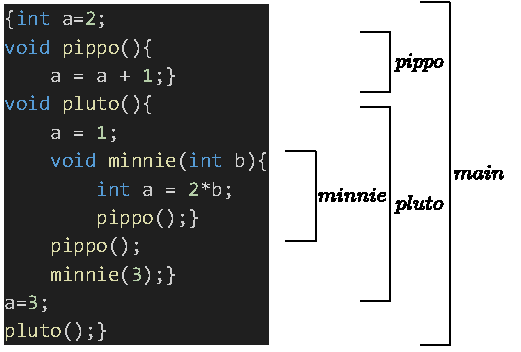
\includegraphics[width=\textwidth]{img/ex3-1.pdf}
		\end{center}
	\end{minipage}
	\begin{minipage}{.3\textwidth}
		\begin{equation*}
			\begin{array}{rcl}
				Sd\left(main\right) &=& 0 \\
				Sd\left(pippo\right) &=& 1 \\
				Sd\left(pluto\right) &=& 1 \\
				Sd\left(minnie\right) &=& 2 \\
			\end{array}
		\end{equation*}
	\end{minipage}\newline
	
	\noindent
	\textbf{\emph{Passo 2:}} si procede con l'esecuzione del codice, calcolando, ad ogni chiamata, i link statici e mostrando come vengono risolti i riferimenti non locali. Si ricorda che la formula per calcolare i link statici è:
	\begin{equation*}
		k = Sd(Ch) - Sd(P) + 1
	\end{equation*}
	Un link dinamico punta sempre al chiamante, così da formare la catena dinamica, mentre un link statico dipende dalla formula soprastante.
	
	La profondità statica (Sd, \emph{static deep}) del chiamante $Ch$, meno la profondità statica del chiamato, cioè la procedura $P$, più uno. Inoltre, la formula per calcolare i riferimenti non locali è:
	\begin{equation*}
		N = Sd(P) - Sd(D)
	\end{equation*}
	Numero di volte necessario per risalire la catena statica è dato dalla differenza tra la profondità statica della procedura in cui viene utilizzato l'identificatore ($Sd(P)$), meno la profondità statica della procedura $D$ che definisce tale identificatore ($Sd(D)$).
	
	Infine, con $CS$ si indica l'abbreviazione di Catena Statica, ovvero la catena di link statici che collegano le istanze del RdA.\newpage
	\begin{enumerate}
		\item $\mathbf{main}$ invoca la funzione $\mathbf{pluto}$.
		\begin{equation*}
			\begin{array}{rcl}
				\text{Link statico} &\rightarrow& Sd(main) - Sd(pluto) + 1 = 0 - 1 + 1 = 0 \\ [.3em]
				&\Rightarrow& CS\left(pluto\right) = indirizzo\left(main\right) \\ [.3em]
				\text{Riferimento non locale }a &\rightarrow& N = Sd(pluto) - Sd(main) = 1 - 0 = 1
			\end{array}
		\end{equation*}
		\begin{figure}[!htp]
			\centering
			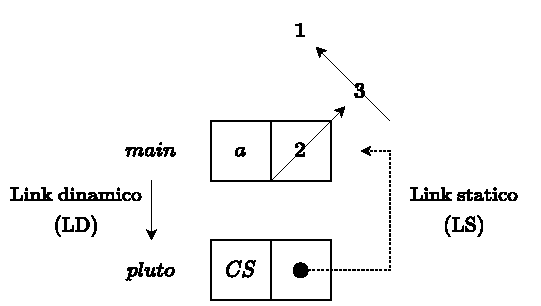
\includegraphics[width=.6\textwidth]{img/ex3-2.pdf}
			\caption*{Evoluzione della memoria.}
		\end{figure}\newpage
		
		\item $\mathbf{pluto}$ invoca la funzione $\mathbf{pippo}$.
		\begin{equation*}
			\begin{array}{rcl}
				\text{Link statico} &\rightarrow& Sd(pluto) - Sd(pippo) + 1 = 1 - 1 + 1 = 1 \\ [.3em]
				&\Rightarrow& CS(pippo) = indirizzo(CS(pluto)) \\ [.3em]
				& &\phantom{ CS(pippo) }= indrizzo(main) \\ [.3em]
				\text{Riferimento non locale }a &\rightarrow& Sd(pippo) - Sd(main) = 1 - 0 = 1
			\end{array}
		\end{equation*}
		\begin{figure}[!htp]
			\centering
			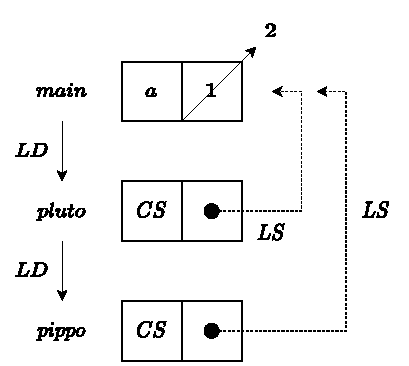
\includegraphics[width=.6\textwidth]{img/ex3-3.pdf}
			\caption*{Evoluzione della memoria.}
		\end{figure}\newpage
		
		\item $\mathbf{pluto}$ invoca la funzione $\mathbf{minnie}$.
		\begin{equation*}
			\begin{array}{rcl}
				\text{Link statico} &\rightarrow& Sd(pluto) - Sd(minnie) + 1 = 1 - 2 + 1 = 0 \\ [.3em]
				&\Rightarrow& CS(minnie) = indirizzo(pluto) \\ [.3em]
				\text{Riferimento non locale} &\rightarrow& \text{nessuno}
			\end{array}
		\end{equation*}
		\begin{figure}[!htp]
			\centering
			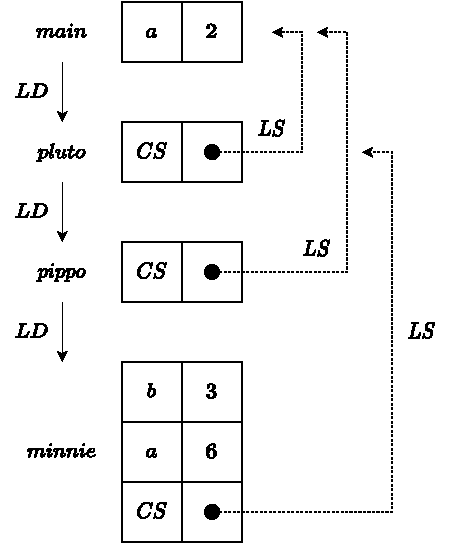
\includegraphics[width=.6\textwidth]{img/ex3-4.pdf}
			\caption*{Evoluzione della memoria.}
		\end{figure}\newpage
		
		\item $\mathbf{minnie}$ invoca la funzione $\mathbf{pippo}$.
		\begin{equation*}
			\begin{array}{rcl}
				\text{Link statico} &\rightarrow& Sd(minnie) - Sd(pippo) + 1 = 2 - 1 + 1 = 2 \\ [.3em]
				&\Rightarrow& CS(pippo) = indirizzo(CS(CS(minnie))) \\ [.3em]
				&&\phantom{ CS(pippo) } = indirizzo(CS(pluto)) \\ [.3em]
				&&\phantom{ CS(pippo) } = indirizzo(main) \\ [.3em]
				\text{Riferimento non locale }a &\rightarrow& N = Sd(pippo) - Sd(main) = 1-0 = 1
			\end{array}
		\end{equation*}
		\begin{figure}[!htp]
			\centering
			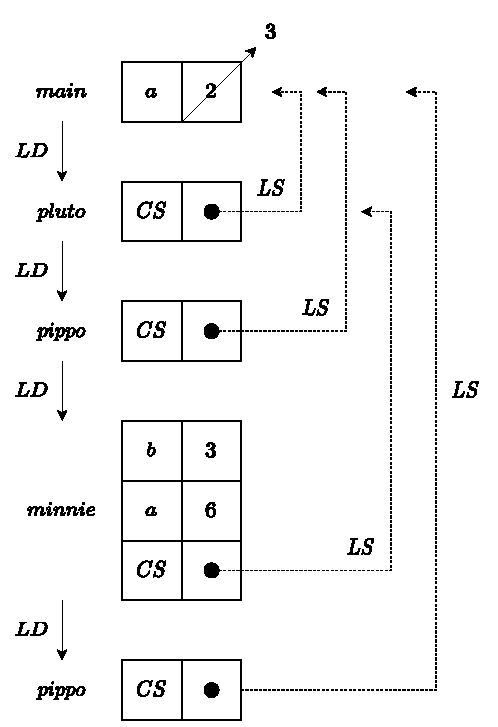
\includegraphics[width=.6\textwidth]{img/ex3-5.pdf}
			\caption*{Evoluzione della memoria.}
		\end{figure}
	\end{enumerate}\newpage
	
	\begin{center}
		\textbf{\emph{\underline{Scope dinamico}}}
	\end{center}
	
	\noindent
	Ogni \underline{aggiornamento} della tabella, ovvero ogni aggiornamento della lista di elementi per gli identificatori, viene eseguita inserendo in cima l'ultima dichiarazione eseguita.\newline
	
	\noindent
	\textbf{Chiamata principale del \emph{main}}. Variabile inizializzata a 2 e poi aggiornata al valore 3:
	\begin{figure}[!htp]
		\centering
		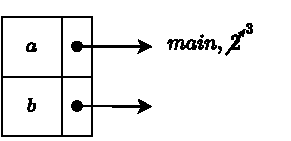
\includegraphics[width=.5\textwidth]{img/ex3-6.pdf}
	\end{figure}
	
	\noindent
	$\mathbf{main}$\textbf{ invoca }$\mathbf{pluto}$. Aggiornamento del valore della variabile $a$ con il valore 3:
	\begin{figure}[!htp]
		\centering
		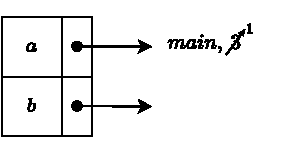
\includegraphics[width=.5\textwidth]{img/ex3-7.pdf}
	\end{figure}
	
	\noindent
	$\mathbf{pluto}$\textbf{ invoca }$\mathbf{pippo}$. Incremento di $1$ del valore della variabile $a$, quindi $1+1 = 2$:
	\begin{figure}[!htp]
		\centering
		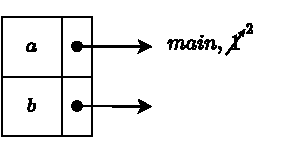
\includegraphics[width=.5\textwidth]{img/ex3-8.pdf}
	\end{figure}
	
	\noindent
	Ritorno da $\mathbf{pippo}$:
	\begin{figure}[!htp]
		\centering
		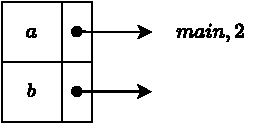
\includegraphics[width=.5\textwidth]{img/ex3-9.pdf}
	\end{figure}\newpage
	
	\noindent
	$\mathbf{pluto}$\textbf{ invoca }$\mathbf{minnie}$. Il parametro $b$ assume il valore $3$, viene aggiornata la lista degli elementi per l'identificatore $a$ inserendo la moltiplicazione tra $b$ e $2$, cioè $2 \times b = 2 \times 3 = 6$:
	\begin{figure}[!htp]
		\centering
		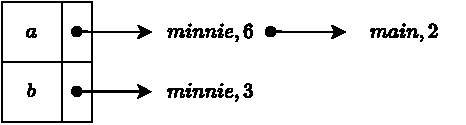
\includegraphics[width=.8\textwidth]{img/ex3-010.pdf}
	\end{figure}
	
	\noindent
	$\mathbf{minnie}$\textbf{ invoca }$\mathbf{pippo}$. Ancora una volta, $pippo$ incrementa la variabile $a$, ma questa volta si riferisce a $minnie$, a causa dello scoping dinamico (shallow binding):
	\begin{figure}[!htp]
		\centering
		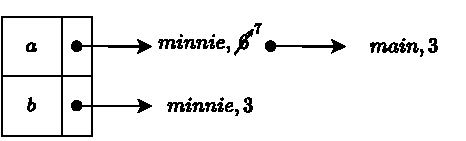
\includegraphics[width=.8\textwidth]{img/ex3-011.pdf}
	\end{figure}
	
	\noindent
	Ritorno da $\mathbf{pippo}$:
	\begin{figure}[!htp]
		\centering
		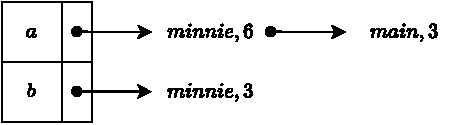
\includegraphics[width=.8\textwidth]{img/ex3-012.pdf}
	\end{figure}
	
	\noindent
	Ritorno da $\mathbf{minnie}$. Vengono rimossi gli elementi $a,b$ che si riferiscono a $minnie$ poiché la chiamata è stata conclusa:
	\begin{figure}[!htp]
		\centering
		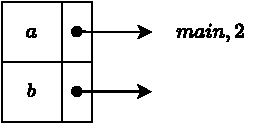
\includegraphics[width=.5\textwidth]{img/ex3-013.pdf}
	\end{figure}
	
	\noindent
	La CRT dopo il ritorno da $\mathbf{pluto}$ è identico alla figura soprastante.
	
	\newpage
	
	% 2023-02-01
	% 2022-09-19
	% 2022-09-19
	% 2020-02-03
	
	\subsection{Tipologia codice 2}
	
	% 2022-02-24
	\newpage
	
	\subsection{Tipologia codice 3}
	
	% 2021-07-13
	\newpage
	
	\subsection{Tipologia codice 4}
	
	% 2021-02-25
	% 2020-02-20
	\newpage
	
	\subsection{Tipologia codice 5}
	
	% 2021-02-08
	\newpage
	
	\subsection{Tipologia codice 6}
	
	% 2020-09-24
	\newpage
	
	\subsection{Tipologia codice 7}
	
	% 2020-09-24
	\newpage
	
	\subsection{Tipologia codice 8}
	
	% 2020-02-04
	\newpage
	
	\subsection{Tipologia codice 9}
	% 2023-06-28
	\textcolor{Red3}{\textbf{\emph{Si consideri il programma sulla destra. Si dica cosa viene calcolato dall'assegnamento in caso di scoping statico (mostrando come vengono calcolati i link statici e come vengono risolti riferimenti non locali) e in caso di scoping dinamico (mostrando l'evoluzione della tabella centrale dei riferimenti (CRT) e come vengono risolti riferimenti non locali).}}}
	\lstinputlisting[language=C]{code/ex3-9.c}
	\textcolor{Green4}{\textbf{\emph{\underline{Risposta}}}}\newline
	
	\noindent
	Esistono due tipologie di scoping:
	\begin{itemize}
		\item Statico, in cui un nome non locale è risolto nel blocco che lo racchiude;
		
		\item Dinamico, in cui un nome non locale è risolto nella chiamata attivata più di recente e non ancora terminata.
	\end{itemize}
	La tabella centrale dei riferimenti (CRT) si riferisce allo scope dinamico. Quest'ultimo può essere implementato, a livello pratico, tramite una tecnica chiamata Shallow Access. Essa consente di avere una struttura dati centrale contenente le variabili locali. Dunque, la tabella CRT ha tre caratteristiche principali:
	\begin{itemize}
		\item Ogni entry corrisponde ad una variabile nel programma;
		
		\item Ogni entry ha un puntatore ad una lista di elementi;
		
		\item Ogni lista di elementi contiene informazioni necessarie ad accedere ad un eventuale ambiente di riferimento
	\end{itemize}\newpage
	
	\begin{center}
		\textbf{\emph{\underline{Scoping statico}}}
	\end{center}
	
	\noindent
	\textbf{\emph{Passo 1:}} si calcola la profondità statica ($Sd$, Static deep) di ciascuna funzione presente all'interno del programma. La profondità statica indica la profondità di annidamento della definizione della procedura corrispondente al Record di Attivazione (RdA), i.e. Stack/Pila).\newline
	
	\noindent
	\begin{minipage}{.7\textwidth}
		\begin{center}
			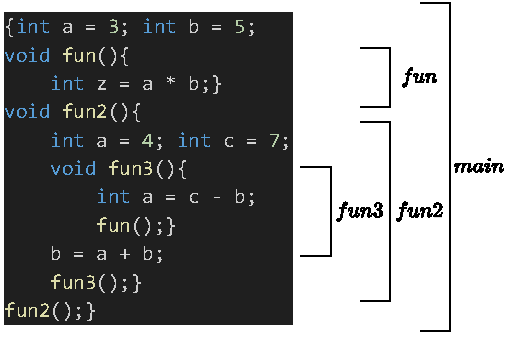
\includegraphics[width=\textwidth]{img/ex3-014.pdf}
		\end{center}
	\end{minipage}
	\begin{minipage}{.3\textwidth}
		\begin{equation*}
			\begin{array}{rcl}
				Sd\left(main\right) &=& 0 \\
				Sd\left(fun\right) &=& 1 \\
				Sd\left(fun2\right) &=& 1 \\
				Sd\left(fun3\right) &=& 2 \\
			\end{array}
		\end{equation*}
	\end{minipage}\newline
	
	\noindent
	\textbf{\emph{Passo 2:}} si inizia ad analizzare il codice. Come richiesto dall'esercizio, si espone il calcolo dei link statici:
	\begin{equation*}
		k = Sd(Ch) - Sd(P) + 1
	\end{equation*}
	Con $Sd(Ch)$ che rappresenta la profondità statica del chiamante, $Sd(P)$ la profondità statica del programma invocato e $k$ la profondità (def. di \emph{static deep}). L'insieme dei link statici forma una catena statica (CS), ovvero un collegamento delle varie istanze del RdA. Al contrario, i link dinamici (DL, \emph{dynamic link}) puntano sempre al chiamante e formano la catena dinamica;\newline
	Il calcolo di eventuali riferimenti non locali:
	\begin{equation*}
		N = Sd(P) - Sd(D)
	\end{equation*}
	Con $Sd(P)$ che rappresenta la profondità statica della procedura che sta utilizzando il riferimento non locale, $Sd(D)$ che rappresenta la profondità statica della procedura in cui è stato definito il riferimento, $N$ che rappresenta il numero di volte necessarie per risalire la catena statica.\newpage
	
	\noindent
	$\mathbf{main}$ invoca la funzione $\mathbf{fun2}$.
	\begin{equation*}
		\begin{array}{rcl}
			\text{Link statico} &\rightarrow& Sd(main) - Sd(fun2) + 1 = 0 - 1 + 1 = 0 \\ [.3em]
			&\Rightarrow& CS(fun2) = indirizzo(main) \\ [.3em]
			\text{Riferimento non locale }b &\rightarrow& N = Sd(fun2) - Sd(main) = 1 - 0 = 1
		\end{array}
	\end{equation*}
	\begin{figure}[!htp]
		\centering
		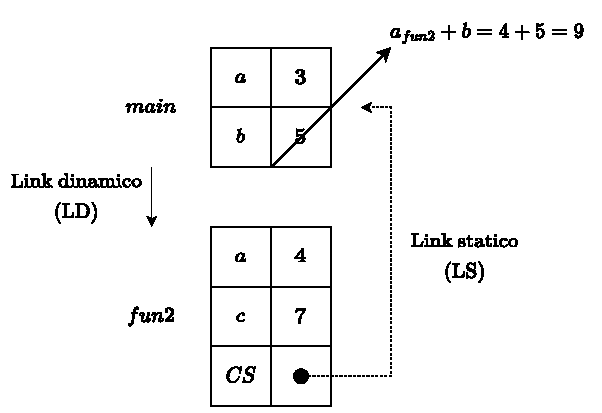
\includegraphics[width=\textwidth]{img/ex3-015.pdf}
	\end{figure}\newpage
	
	$\mathbf{fun2}$ invoca la funzione $\mathbf{fun3}$.
	\begin{equation*}
		\begin{array}{rcl}
			\text{Link statico} &\rightarrow& Sd(fun2) - Sd(fun3) + 1 = 1 - 2 + 1 = 0 \\ [.3em]
			&\Rightarrow& CS(fun3) = indirizzo(fun2) \\ [.3em]
			\text{Riferimento non locale }c &\rightarrow& N = Sd(fun3) - Sd(fun2) = 2 - 1 = 1 \\ [.3em]
			\text{Riferimento non locale }b &\rightarrow& N = Sd(fun3) - Sd(main) = 2 - 0 = 2
		\end{array}
	\end{equation*}
	\begin{figure}[!htp]
		\centering
		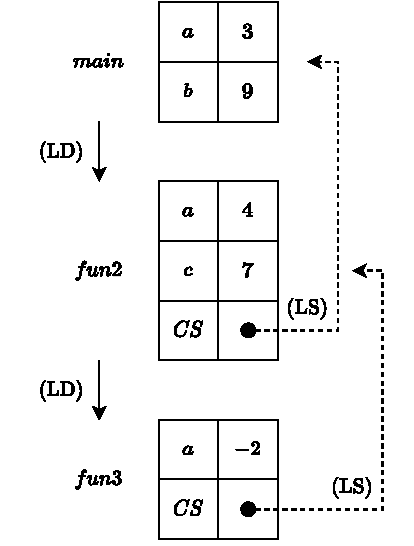
\includegraphics[width=.6\textwidth]{img/ex3-016.pdf}
	\end{figure}\newpage
	
	\noindent
	$\mathbf{fun3}$ invoca la funzione $\mathbf{fun}$.
	\begin{equation*}
		\begin{array}{rcl}
			\text{Link statico} &\rightarrow& Sd(fun3) - Sd(fun) + 1 = 2 - 1 + 1 = 2 \\ [.3em]
			&\Rightarrow& CS(fun) = indirizzo(CS(CS(fun3))) \\ [.3em]
			&&\phantom{ CS(fun)} = indirizzo(CS(fun2)) \\ [.3em]
			&&\phantom{ CS(fun)} = indirizzo(main) \\ [.3em]
			\text{Riferimento non locale }a &\rightarrow& N = Sd(fun) - Sd(main) = 1 - 0 = 1 \\ [.3em]
			\text{Riferimento non locale }b &\rightarrow& N = Sd(fun) - Sd(main) = 1 - 0 = 1
		\end{array}
	\end{equation*}
	\begin{figure}[!htp]
		\centering
		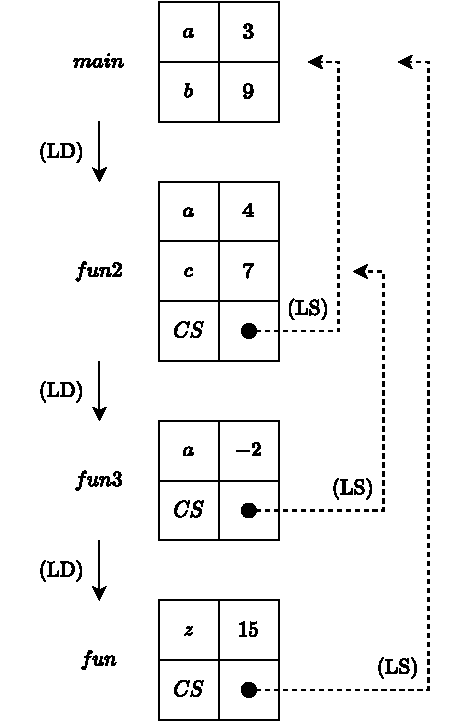
\includegraphics[width=.7\textwidth]{img/ex3-017.pdf}
	\end{figure}\newpage
	
	\begin{center}
		\textbf{\emph{\underline{Scoping dinamico}}}
	\end{center}
	
	\noindent
	Ogni \underline{aggiornamento} della tabella CRT, ovvero ogni aggiornamento della lista di elementi degli identificatori, viene effettuata inserendo in cima l'ultima dichiarazione eseguita.\newline
	
	\noindent
	\textbf{Chiamata principale del }$\mathbf{main}$. Inizializzazione delle variabili $a,b$:
	\begin{figure}[!htp]
		\centering
		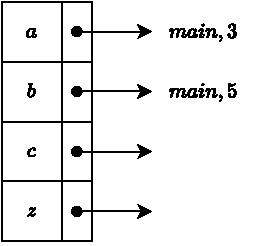
\includegraphics[width=.4\textwidth]{img/ex3-018.pdf}
	\end{figure}
	
	\noindent
	$\mathbf{main}$\textbf{ invoca }$\mathbf{fun2}$. Vengono inizializzate due variabili locali, quindi si aggiungono alla lista degli elementi dei rispettivi identificatori. Inoltre, la variabile $b$, che è stata dichiarata nel $main$, viene aumentata di $4$:
	\begin{figure}[!htp]
		\centering
		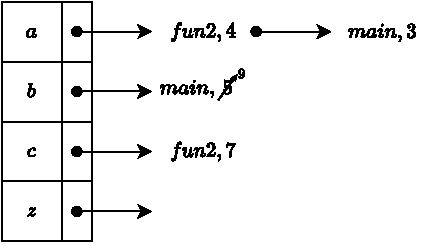
\includegraphics[width=.7\textwidth]{img/ex3-019.pdf}
	\end{figure}
	
	\noindent
	$\mathbf{fun2}$\textbf{ invoca }$\mathbf{fun3}$. Viene inizializzata una variabile locale, quindi si aggiunge alla lista degli elementi dell'identificatore $a$:
	\begin{figure}[!htp]
		\centering
		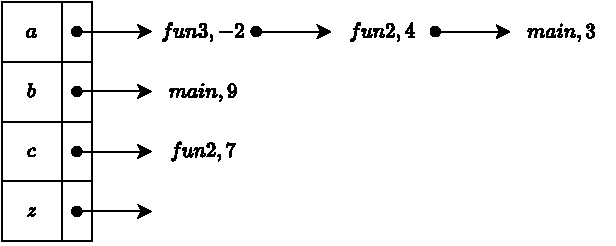
\includegraphics[width=.9\textwidth]{img/ex3-020.pdf}
	\end{figure}\newpage
	
	\noindent
	$\mathbf{fun3}$\textbf{ invoca }$\mathbf{fun}$. Viene inizializzata una variabile locale, quindi si aggiunge alla lista degli elementi dell'identificatore $z$:
	\begin{figure}[!htp]
		\centering
		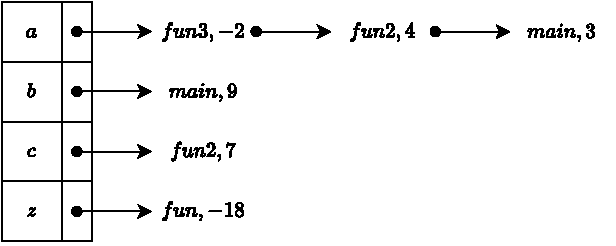
\includegraphics[width=.9\textwidth]{img/ex3-021.pdf}
	\end{figure}
	
	\noindent
	\textbf{Ritorno di }$\mathbf{fun}$\textbf{ in }$\mathbf{fun3}$. La lista degli elementi dell'identificatore $z$ viene aggiornata eliminando l'elemento riferito alla procedura $fun$ (a causa della sua terminazione):
	\begin{figure}[!htp]
		\centering
		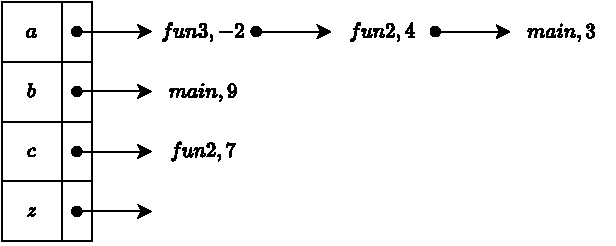
\includegraphics[width=\textwidth]{img/ex3-022.pdf}
	\end{figure}
	
	\noindent
	\textbf{Ritorno di }$\mathbf{fun3}$\textbf{ in }$\mathbf{fun2}$. La lista degli elementi dell'identificatore $a$ viene aggiornata eliminando l'elemento riferito alla procedura $fun3$ (sempre a causa della terminazione):
	\begin{figure}[!htp]
		\centering
		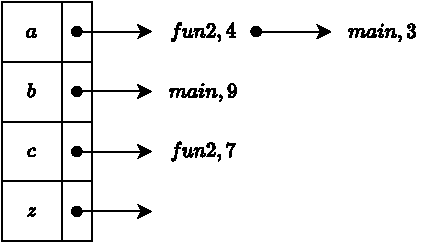
\includegraphics[width=.7\textwidth]{img/ex3-023.pdf}
	\end{figure}\newpage
	
	\noindent
	\textbf{Ritorno di }$\mathbf{fun2}$\textbf{ in }$\mathbf{main}$. Si libera $a,c$:
	\begin{figure}[!htp]
		\centering
		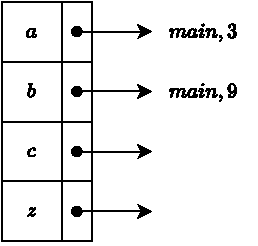
\includegraphics[width=.4\textwidth]{img/ex3-024.pdf}
	\end{figure}\newpage
	
	\section{Esercizio 4 - Scoping (statico/dinamico) e Binding}
	
	\subsection{Regole di scoping e di binding}
	
	\textcolor{Red3}{\textbf{\emph{Spiegare dove e perché nel programma è necessario parlare di regole di scoping, e dove (e perché) anche di regole di binding. Si dica quale risulta essere il valore finale di $z$ nelle varie situazioni, ovvero con: (1) scoping statico; (2) scoping dinamico e deep-binding; (3) shallow-binding (e scoping dinamico).}}}
	\lstinputlisting[language=C]{code/ex4-1.c}
	
	\noindent
	\textcolor{Green4}{\textbf{\emph{\underline{Risposta}}}}\newline
	
	\noindent
	In questo caso, ma vale in generale, le regole di scope e di binding sono necessarie quando la procedura contiene un ambiente non locale. Precisamente:
	\begin{itemize}
		\item Le regole di scoping poiché è necessario risolvere riferimenti non locali;
		
		\item Le regole di binding poiché le chiamate a funzione hanno tra i parametri delle funzioni.
	\end{itemize}
	Ovviamente la premessa è che le procedure abbiano ambienti non locali.\newline
	
	\noindent
	La definizione di \emph{scoping} è stata data in modo esaustivo nell'esercizio 3 (capitolo 3).\newline
	
	\noindent
	Con \emph{binding} si intende l'associazione tra un nome e un valore. Quest'ultimo non deve per forza essere un valore numerico, ma può anche essere una stringa, una funzione, una lista, ecc.
	\begin{itemize}
		\item Deep-binding, viene utilizzato l'ambiente valido al momento della definizione del legame tra parametro attuale e formale;
		
		\item Shallow-binding, gli ambienti da tenere in considerazione sono due:
		\begin{itemize}
			\item L'ambiente valido al momento della creazione del legame tra parametro attuale e parametro formale;
			
			\item L'ambiente valido al momento della chiamata del parametro attuale attraverso il parametro formale.
		\end{itemize}
	\end{itemize}
	Il parametro formale è un parametro noto nella definizione della funzione. Invece, il parametro attuale è quello che viene passato effettivamente alla funzione quando viene invocata.\newpage
	
	\begin{center}
		\textbf{\emph{\underline{Scoping statico}}}
	\end{center}
	
	\noindent
	All'invocazione di $f\left(b\right)$ (riga 6), la funzione $pluto$ passa come parametro la sua variabile locale $b$, ovvero $5$. La funzione $f$, parametro formale, è legata al parametro attuale $pippo$. Quindi, nel corpo di $pippo$ viene fatto il calcolo:
	\begin{equation*}
		a + b - in
	\end{equation*}
	Dove $a$ si riferisce alla $a$ del $main$, ovvero la variabile a riga 1 con valore $4$; dove $b$ si riferisce alla $b$ del $main$, ovvero la variabile a riga 1 con valore $3$; dove $in$ si riferisce al parametro formale, quindi corrisponde a $5$, ovvero il valore che gli è stato passato.
	\begin{equation*}
		4 + 3 - 5 = 2
	\end{equation*}
	Il valore $2$ viene ritornato. Quindi, alla riga 6 viene effettuata la somma tra $2$ e la variabile locale $a$. Il risultato che viene ritornato dalla funzione $pluto$, che corrisponde al risultato della variabile $z$, è $2+6=8$.
	
	\begin{center}
		\textbf{\emph{\underline{Scoping dinamico e deep-binding}}}
	\end{center}
	
	\noindent
	All'invocazione della funzione $f(b)$ (riga 6), la funzione $pluto$ passa come parametro la sua variabile locale $b$, ovvero $5$. La funzione $f$, parametro formale, è legata al parametro attuale $pippo$. Quindi, nel corpo di $pippo$ viene fatto il calcolo:
	\begin{equation*}
		a+b-in
	\end{equation*}
	\begin{itemize}
		\item $a$ considera l'ambiente al momento della definizione. Quindi, si prende il valore $4$ del main;
		
		\item $b$ sempre considerando l'ambiente al momento della definizione, si prende il valore $2$;
		
		\item $in$ è sempre $5$.
	\end{itemize}
	\begin{equation*}
		4 + 2 - 5 = 1
	\end{equation*}
	Quindi, viene tornato il valore $1$ alla funzione $pluto$. Quest'ultima ritorna la somma tra $1$ e la variabile locale $a$, cioè $1+6=7$. Quindi il valore finale di $z$ è $7$.
	
	\begin{center}
		\textbf{\emph{\underline{Scoping dinamico e shallow-binding}}}
	\end{center}
	
	\noindent
	Il procedimento è lo stesso dei precedenti. L'unica differenza è nel calcolo che esegue la funzione $pippo$, che ovviamente si ripercuote sul valore ritornato dalla funzione $pluto$.
	\begin{equation*}
		a + b - in
	\end{equation*}
	Viene preso il valore $6$ per $a$, quello della funzione $pluto$; viene preso il valore $5$ per $b$, quello della funzione $pluto$; viene preso il valore $5$ per $in$, il valore passato come parametro da $pluto$.
	\begin{equation*}
		6 + 5 - 5 = 6
	\end{equation*}
	Il valore di $z$ sarà:
	\begin{equation*}
		6 + 6 = 12
	\end{equation*}
	Poiché si prende $a$ come variabile locale.\newpage
	
	\subsection{Codice da inserire in caso di scoping statico/dinamico}
	
	\subsubsection{Tipologia di codice 1}
	% 2022-02-24
	\newpage
	
	\subsubsection{Tipologia di codice 2}
	% 2023-06-28
	% 2020-02-20
	
	\textcolor{Red3}{\textbf{\emph{Si consideri lo schema del seguente codice, nel quale vi sono due buchi indicati rispettivamente con (*) e (**). Si dia il codice da inserire al posto di (*) e (**) in modo tale che:}}}
	\begin{enumerate}[label=(\alph*)]
		\item \textcolor{Red3}{\textbf{\emph{Se il linguaggio usato adotta lo scope statico, le due chiamate alla procedura pluto assegnino a $x$ lo stesso valore;}}}
		
		\item \textcolor{Red3}{\textbf{\emph{Se il linguaggio usato adotta lo scope dinamico, le due chiamate alla procedura pluto assegnino a $x$ valori diversi.}}}
	\end{enumerate}
	\textcolor{Red3}{\textbf{\emph{Si descrivano dettagliatamente le scelte fatte e si descriva cosa avviene a tempo di esecuzione in entrambi i casi e perché.}}}
	\lstinputlisting[language=C]{code/ex4-2.c}
	
	\noindent
	\textcolor{Green4}{\textbf{\emph{\underline{Risposta}}}}\newline
	
	\noindent
	La differenza tra scoping statico e scoping dinamico è stata data nell'esercizio 3. Si procede dunque con la soluzione dei due codici nelle due casistiche.\newline
	
	\noindent
	Si riscrive il codice per avere una spaziatura migliore:
	\lstinputlisting[language=C]{code/ex4-3.c}
	\begin{itemize}
		\item (*) il codice da inserire è:
		\begin{lstlisting}[language=C]
i = 0;
int y = 2;
void pluto(){
	return y;
}\end{lstlisting}
		
		\item (**) il codice da inserire è:
		\begin{lstlisting}[language=C]
y = i;
x = 3;\end{lstlisting}
	\end{itemize}\newpage
	
	\noindent
	Quindi, il codice finale diventa:
	\lstinputlisting[language=C]{code/ex4-4.c}
	Alla partenza del codice, viene creata una variabile $y$ e gli viene assegnato il valore $2$. Alla chiamata della funzione $pippo$, viene dichiarata un'altra variabile $y$ e gli viene assegnato il valore di $i$ che inizialmente è $0$ e poi $1$. Alla variabile $x$, presente nel $main$ viene assegnato il valore $3$. Successivamente, viene chiamata la funzione $pluto$ e qua i risultati sono differenti:
	\begin{itemize}
		\item Scope statico:
			\begin{itemize}
				\item $i = 0$: la funzione $pluto$ ritorna il valore $2$, ovvero quello del $main$. Quindi la $x$ diventa $2 + 3 = 5$.
				
				\item $i = 1$: la funzione $pluto$ ritorna nuovamente il valore $2$ e la somma è di nuovo $5$ poiché la $x$ con il ciclo $i=0$ è stata aggiornata a $5$, ma con il ciclo $i=1$ è ritornata a $3$ grazie alla dichiarazione a riga 10.
			\end{itemize}
		
		\item Scope dinamico:
			\begin{itemize}
				\item $i = 0$: la funzione $pluto$ ritorna il valore $0$, ovvero quello uguale alla variabile $i$. Quindi la $x$ diventa $0 + 3 = 3$.
				
				\item $i = 1$: la funzione $pluto$ ritorna il valore $1$, ovvero quello uguale alla variabile $i$. Quindi la $x$ diventa $1 + 3 = 4$. Il fatto che la $x$ non sia stata aggiornata è dovuta allo stesso motivo spiegato nello scope statico.
			\end{itemize}
	\end{itemize}\newpage
	
	\subsubsection{Tipologia di codice 3}
	% 2020-09-24
	% 2020-02-24
	\newpage
	
	
	\section{Esercizio 5 - Ricorsione e passaggio di parametri}
	
	\subsection{Ricorsione e ricorsione in coda}
	
	\textcolor{Red3}{\textbf{\emph{Definire brevemente il concetto di ricorsione e di ricorsione in coda. Si consideri il programma ricorsivo a destra e si descriva che cosa calcola mostrando anche il calcolo sulla lista $\left(2,4,6\right)$. Trasformare quindi tale programma in un programma ricorsivo in coda. Mostrare poi il funzionamento dell'algoritmo fornito sulla lista $\left(2,4,6\right)$.}}}\newline
	
	\noindent
	\textcolor{Red3}{\textbf{\emph{NOTA: Data una lista list, length(list) restituisce la sua lunghezza, car(list) restituisce il primo elemento, cdr(list) restituisce tutta la lista tranne il primo elemento, concat concatena due liste (se un elemento non è una lista, concat lo converte prima in lista). () è la lista vuota.}}}
	\lstinputlisting[language=C]{code/ex5-1.c}
	
	\noindent
	\textcolor{Green4}{\textbf{\emph{\underline{Risposta}}}}\newline
	
	\noindent
	Una funzione viene definita \textbf{ricorsiva} se viene definita in termini di se stessa. Le funzioni ricorsive derivano direttamente dalle definizioni di induzione, tuttavia rimangono concetti diversi:
	\begin{itemize}
		\item L'induzione è un concetto matematico ed è sempre ben fondata;
		
		\item L'induzione \dquotes{informatica} può divergere. Ovvero, un programma potrebbe non terminare mai (i.e. \textsf{while(true)\{x=x\}}).
	\end{itemize}
	Una chiamata di una funzione $g$ in una funzione $f$ viene definita \dquotes{in coda}, se la funzione $f$ restituisce il valore restituito dalla funzione $g$ senza ulteriore computazione. Se ne deduce, che una funzione ricorsiva viene chiamata \dquotes{\textbf{funzione ricorsiva in coda}} quando contiene solo chiamate ricorsive in coda.
	
	\begin{center}
		\textbf{\emph{\underline{Calcolo ricorsione}}}
	\end{center}
	
	\noindent
	Considerando la lista $\left(2,4,6\right)$, la funzione ricorsiva esegue le seguenti operazioni:
	\begin{equation*}
		\begin{array}{llll}
			&&& = (18,12,6)\\ [.6em]
			function(2,4,6) &\longrightarrow& concat\left((4,6), 2*3\right);& \uparrow 7\degree\\ [.6em]
			&& 1\degree\downarrow& (18, 12) \\ [.6em]
			&& concat\left((6), 4*3\right);& \uparrow 6\degree \\ [.6em]
			&& 2\degree\downarrow& \uparrow (18) \\ [.6em]
			&& concat\left((), 6*3\right);& \uparrow 5\degree \\ [.6em]
			&& 3\degree\downarrow& \uparrow() \\ [.6em]
			&& return();& \uparrow 4\degree
		\end{array}
	\end{equation*}
	L'\textbf{obbiettivo} della funzione ricorsiva è invertire l'ordine della lista e moltiplicare ciascun valore per 3. In caso di lista vuota, il risultato è una lista vuota.
	
	\begin{center}
		\textbf{\emph{\underline{Trasformazione da ricorsione a ricorsione in coda}}}
	\end{center}
	
	\noindent
	La trasformazione da ricorsione a ricorsione in coda può avvenire se si definisce una funzione che restituisce il valore di un'altra funzione senza altre computazioni. Quindi, si definisce la funzione $functionrc$ che esegue le stesse cose della funzione $function$ originale, ma con un parametro in più, ovvero il risultato parziale. Questo consente di non elaborare valori dopo le chiamate ricorsive. Mentre la funzione $function$ (nuova, non l'originale) che prende come parametro una lista e ritorna come risultato la computazione della ricorsione senza eseguire ulteriori operazioni:
	\lstinputlisting[language=C]{code/ex5-2.c}
	Considerando la lista $\left(2,4,6\right)$, la ricorsione in coda esegue le seguenti operazioni:
	\begin{equation*}
		\begin{array}{llll}
			&&& = (18,12,6)\\ [.6em]
			function((2,4,6), ()) &\longrightarrow& functionrc\left((2,4,6), ()\right);& \uparrow 9\degree\\ [.6em]
			&& 1\degree\downarrow () & (18, 12, 6) \\ [.6em]
			&& functionrc\left((4,6), 2*3\right);& \uparrow 8\degree \\ [.6em]
			&& 2\degree\downarrow (6)& \uparrow (18, 12, 6) \\ [.6em]
			&& functionrc\left((6), 4*3\right);& \uparrow 7\degree \\ [.6em]
			&& 3\degree\downarrow (12, 6)& \uparrow(18, 12, 6) \\ [.6em]
			&& functionrc\left((), 6*3\right);& \uparrow 6\degree \\ [.6em]
			&& 4\degree\downarrow (18, 12, 6)& \uparrow(18, 12, 6) \\ [.6em]
			&& return res;& \uparrow 5\degree
		\end{array}
	\end{equation*}
	
	\newpage
	\subsection{Passaggio di parametri: per valore e per riferimento}
	
	\subsubsection{Tipologia di codice 1}
	% 2023-06-28
	
	\subsubsection{Tipologia di codice 2}
	% 2023-02-01
	
	\subsubsection{Tipologia di codice 3}
	% 2021-02-08
	
	\subsubsection{Tipologia di codice 4}
	% 2020-02-04
	
	\section{Esercizio 6 - Regole della semantica dinamica}
	
	\subsection{Derivazioni semantica dinamica}
	
	\subsubsection{Tipologia di memoria 1}
	% 2023-06-28
	
	\subsubsection{Tipologia di memoria 2}
	% 2023-02-01
	% 2022-09-19
	% 2022-02-03
	
	\subsubsection{Tipologia di memoria 3}
	% 2021-02-08
	
	\subsubsection{Vecchi esercizi}
	% 2020-02-20
	% 2020-09-24
	% 2020-02-04
	
	\subsection{Regole della semantica dinamica per il comando condizionale}
	
	% 2022-02-24
	% 2021-02-25
	
	\subsection{Regole della semantica dinamica per l'assegnamento}
	
	% 2021-07-13
\end{document}